% lecture18.tex — Hopf Degree Theorem

\section{Hopf Degree Theorem}

Let $M, N$ be compact, connected, oriented manifolds of the same dimension. The degree of a map $f \colon M \to N$, which counts the number of preimages (with sign) of a generic point in $N$, is a homotopy invariant.

In general, the degree is not a complete invariant, but it turns out to be one when $N = S^n$.

\begin{theorem}{Hopf Degree Theorem}{hopf-degree}
    Let $M$ be a compact, connected, oriented $m$-manifold. Two maps $f_0, f_1 \colon M \to S^m$ are homotopic if and only if
    \[
        \deg f_0 = \deg f_1.
    \]
\end{theorem}

\begin{proof}
    We already know ($\Rightarrow$).

    For ($\Leftarrow$), set $W = M \times I$, and let $f \colon \partial W \to S^m$ be $f_0$ on $M \times \{0\}$ and $f_1$ on $M \times \{1\}$, so that $\deg f = \deg f_1 - \deg f_0 = 0$. The claim then follows from the more general extension theorem below.
\end{proof}

\subsection{Extension Theorem}

\begin{theorem}{Extension Theorem}{extension}
    Let $W$ be a compact, connected, oriented $(m+1)$-manifold with boundary, and let $f \colon \partial W \to S^m$ be a smooth map. Then $f$ extends to a map $F \colon W \to S^m$ with $\partial F = f$ if and only if $\deg f = 0$.
\end{theorem}

\begin{proof}
    We already know ($\Rightarrow$), so let's show ($\Leftarrow$).

    Firstly, any smooth map $f \colon \partial W \to \R^{m+1}$ (without any degree constraint) can be extended to all of $W$. Let $U$ be a collar neighborhood of $\partial W$ and $\widetilde{f} \colon U \xrightarrow{\pi} \partial W \xrightarrow{f} \R^{m+1}$ the projection composed with $f$. Choose a smooth bump $\rho \colon W \to \R$ with $\rho|_{\partial W} \equiv 1$ and $\rho \equiv 0$ outside a compact subset of $U$. Then $F_0 := \rho \widetilde{f}$ extends $f$.

    \begin{center}
    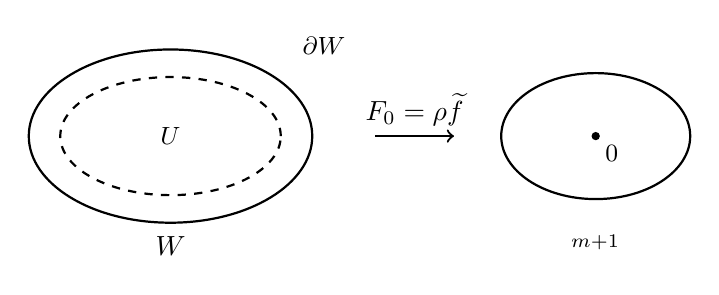
\begin{tikzpicture}[scale=1]
        % W with collar
        \draw[thick] (0,0) ellipse (1.8 and 1.1);
        \draw[thick,dashed] (0,0) ellipse (1.4 and 0.75);
        \node at (0,-1.4) {$W$};
        \node at (0,0) {\small $U$};
        \node at (1.95,1.15) {\small $\partial W$};
        % Arrow
        \draw[->,thick] (2.6,0) -- (3.6,0) node[midway,above] {$F_0 = \rho \widetilde{f}$};
        % Image
        \draw[thick] (5.4,0) ellipse (1.2 and 0.8);
        \fill (5.4,0) circle (1.5pt) node[below right] {\small $0$};
        \node at (5.4,-1.4) {$\R^{m+1}$};
    \end{tikzpicture}
    \end{center}

    After some homotopy in the interior, we may assume that $0 \in \R^{m+1}$ is a regular value of $F_0$, so $F_0^{-1}(0)$ is a finite set of points in $\operatorname{Int}(W)$. We will need:

    \begin{lemma}{Isotopy Lemma}{isotopy}
        Given any two points $x, y$ in a connected manifold $M$, there exists a diffeomorphism $h \colon M \to M$ such that $h(x) = y$ which is isotopic to the identity (i.e.\ each $h_t$ is a diffeomorphism). The isotopy may be taken to be compactly supported.
    \end{lemma}

    Using the isotopy lemma, we may place the finite set $F_0^{-1}(0)$ inside a ball $B \subset \operatorname{Int}(W)$. By the assumption $\deg f = 0$, the directional map $\frac{F_0}{|F_0|}\big|_{\partial B} \colon \partial B \to S^m$ has degree $0$, i.e.\ $F_0|_{\partial B}$ has winding number $0$ around $0 \in \R^{m+1}$. To show that $\frac{F_0}{|F_0|}\big|_{W \setminus \operatorname{Int}(B)}$ extends to all of $W$, it then suffices to prove the following special case of the Hopf degree theorem.
\end{proof}

\subsection{Hopf Theorem for Spheres}

\begin{theorem}{Hopf Theorem for Spheres}{hopf-spheres}
    Any smooth map $f \colon S^m \to S^m$ of degree $0$ is homotopic to a constant map.
\end{theorem}

\begin{proof}
    We proceed by induction on $m$.

    The case $m = 1$ is an exercise (lift the map to a map $\R \to \R$).

    Now assume the claim is true for $m - 1$, and we'll extend it to $m$. Let $p \in S^m$ be a regular value. Using the isotopy lemma, we may assume that the preimage points $f^{-1}(p)$ are contained inside a ball $B \subset S^m$ such that $q \notin f(B)$ for some $q \in S^m$.

    Then we have
    \[
        S^{m-1} \cong \partial B \xrightarrow{f|_{\partial B}} S^m \setminus \{q\} \cong \R^m,
    \]
    where the last identification is some diffeomorphism sending $p$ to $0 \in \R^m$. This composition has winding number $0$ around $0 \in \R^m$, since $\deg f = 0$.

    By the induction hypothesis, $f|_{\partial B}$ is homotopic to a constant map, without crossing $p$. Therefore $f|_{S^m \setminus B} \colon S^m \setminus B \to S^m \setminus \{p\}$ extends to the whole $S^m$, and thus $f \colon S^m \to S^m$ is homotopic to a constant map.
\end{proof}

\subsection{Application: Nowhere-Vanishing Vector Fields}

\begin{theorem}{Existence of Nowhere-Vanishing Vector Fields}{nowhere-vanishing-vf}
    A compact, connected, oriented manifold $M$ possesses a nowhere-vanishing vector field if and only if $\chi(M) = 0$.
\end{theorem}

\begin{proof}
    From Poincar\'e--Hopf, we already know ($\Rightarrow$).

    For the converse ($\Leftarrow$), take a generic vector field $v$ on $M$ with finitely many zeros. Using the isotopy lemma, we may place all the zeros inside some ball $B \subset M$, and since $\chi(M) = 0$, the sum of the indices of the zeros equals $0$.

    It follows that the map $v \colon S^{m-1} \cong \partial B \to \R^m \setminus \{0\}$ has winding number $0$ around $0 \in \R^m$, and by the Hopf degree theorem, it is homotopic to a constant map. Using this homotopy, we can extend $v|_{M \setminus B}$ to a nowhere-vanishing vector field on all of $M$.
\end{proof}

\begin{center}
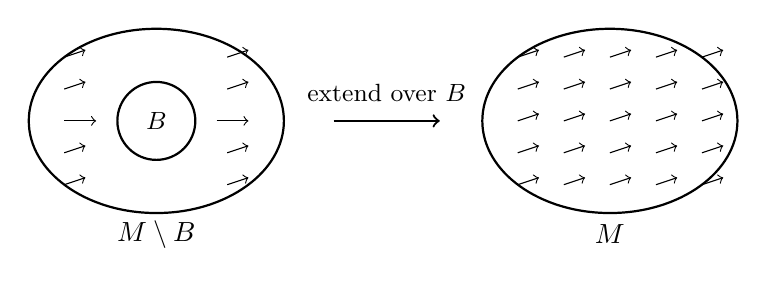
\begin{tikzpicture}[scale=0.9]
    % Left: M with ball B containing zeros
    \draw[thick] (0,0) ellipse (1.8 and 1.3);
    \draw[thick] (0,0) circle (0.55);
    \node at (0,0) {\small $B$};
    \node at (0,-1.6) {$M \setminus B$};
    % Background flow arrows (avoid B)
    \foreach \y in {-0.9, -0.45, 0.45, 0.9} {
        \foreach \x in {-1.3, 1.0} {
            \draw[->,thin] (\x,\y) -- (\x+0.3,\y+0.1);
        }
    }
    \draw[->,thin] (-1.3,0) -- (-0.85,0);
    \draw[->,thin] (0.85,0) -- (1.3,0);
    % Arrow: extend over B
    \draw[->,thick] (2.5,0) -- (4.0,0);
    \node at (3.25,0.4) {\small extend over $B$};
    % Right: full vector field
    \begin{scope}[xshift=6.4cm]
        \draw[thick] (0,0) ellipse (1.8 and 1.3);
        \node at (0,-1.6) {$M$};
        \foreach \y in {-0.9, -0.45, 0, 0.45, 0.9} {
            \foreach \x in {-1.3, -0.65, 0, 0.65, 1.3} {
                \draw[->,thin] (\x,\y) -- (\x+0.3,\y+0.1);
            }
        }
    \end{scope}
\end{tikzpicture}
\end{center}
